% Activate the following line by filling in the right side. If for example the name of the root file is Main.tex, write
% "...root = Main.tex" if the chapter file is in the same directory, and "...root = ../Main.tex" if the chapter is in a subdirectory.
 
%!TEX root =  secondDraft.tex

\chapter[Method]{Method}

\section{Introduction}

This chapter lays out the general method for creating agent-based simulations with automatic Bayesian Networks, as well as how to evaluate these Bayesian Networks.

We can consider an approach in four stages. First, we need a scenario, or set of alternative scenarios, that are to be modelled. These scenarios are written description of crime scenarios that contain the hypothetical events and evidence for these events, as postulated by the prosecutor and defence. 

Second, based on this written description of the scenario(s) to be modelled, an agent-based simulation is created. In the simulation, all events of the scenario need to represented. The simulation can be as granular as desired. The simulation can be run multiple times, so that we can gain an understanding of possible underlying frequency information on the events in the scenario. The frequencies by which events occur in the simulation are collected.

Third, the collected frequencies are then used to automatically build a Bayesian Network on the simulation, using the K2 algorithm. Finally, the generated Bayesian Network is then evaluated based the criteria set out at the end of this chapter.

This four-step process will be explained in this chapter, and illustrated with a running example of a stabbing.

 %The general process of creating simulations to evaluate Bayesian Networks is illustrated in Figure~\ref{pipeline}. 

%\begin{figure}[h]
%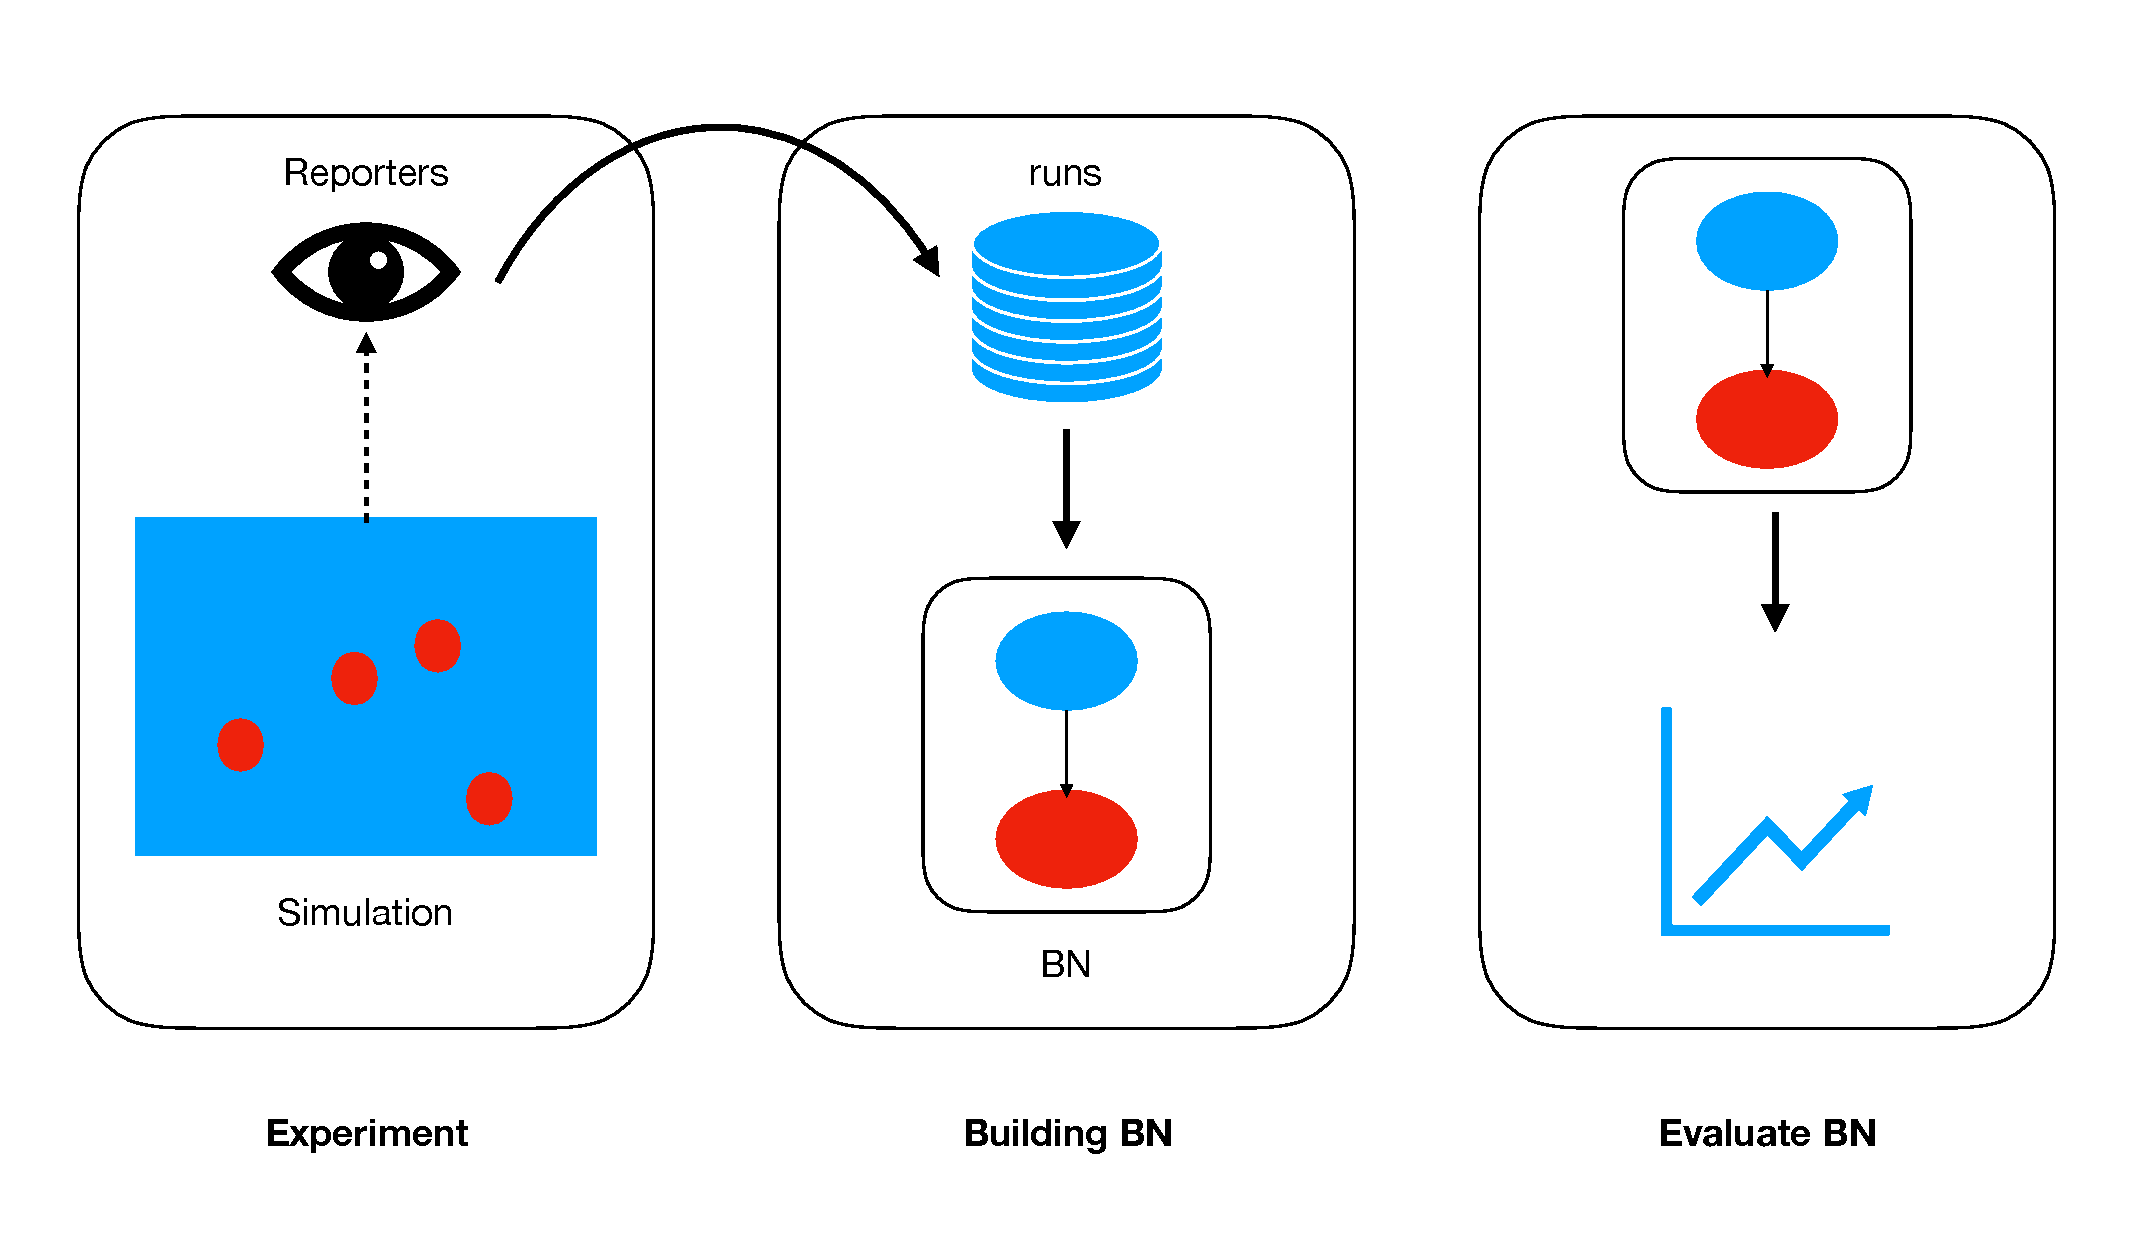
\includegraphics[width=\linewidth]{images/pipeline.pdf}
%\caption{Method for evaluating automatically generated Bayesian Networks from simulations.}
%\label{pipeline}
%\end{figure}

\section{A Scenario}
We start our process with one or more written scenarios. These scenarios can, in the first instance, be obtained from (abridged) court case descriptions. The scenarios should contain all and only those hypothesised events, and the evidence for such events, that are relevant to the case. Both the prosecution and the defence should be able to select relevant events and their evidence. 


\begin{example}
Here we will introduce our running example, loosely based on the first scenario in \citep{vlek2015}: Mark and Jane live together. One day, a neighbour overhears that they've started to fight in the kitchen. Jane grabs a knife, and stabs Mark. Mark dies of the stab wounds, as confirmed by the forensic scientist at the scene. Jane's fingerprints are on the knife.
\end{example}

\section{An Agent-based Simulation}


We need a way to transform the written text descriptions of the events in the scenario to observable events in the simulation. First we identify all relevant actors, objects and places in the scenario. Then we select all relevant events from the written description and attempt to operationalise them in the simulation. This means that we create a way to measure if the events take place within the simulation. This is done by means of `reporters', or random variables. These reporters report whether a given event has taken place within the simulation. 

The process of operationalisation is very subjective and depends entirely on the modeller's assumptions and their time, knowledge or skill constraints. The behaviour of agents, as reflections of actual people, can be modelled in a way that reflect real sociological theories of behaviour (such as in \citet{gerritsen2015}), or with simple rules and a random number generator (such as here). The environment of the simulation can reflect a real-world geography with different affordances, or can be simplified. How a given event is operationalised is essential for the validity of the network: if it is unclear, or disputed, when an event is true in a simulation, the network should not be used.

\begin{example}

We have modelled Jane and Mark as two agents in a simulation (Figure~). The only `psychological' aspect that these agents have, is an anger level, which has 4 escalating states = \{not angry, fighting, grabbing knife, stabbing\}. Jane is quicker to increase to the next anger level. 

\begin{description}
\item[jane\_and\_mark\_fight ]  Both Mark and Jane have an anger level that is higher than `not angry'
\item[jane\_has\_knife ] Jane has an anger level of `grabbing knife' and moved to the location of the knife
\item[jane\_stabs\_mark\_with\_knife ] Jane has an anger level of `stabbing', has the knife, and moved to Mark's position
\item[mark\_dies ] Jane has stabbed Mark, and if a random number generator (uniform, 0, 100) produces a number $>$ 60
\item[E\_neighbour ] Either Mark and Jane have an anger level that is higher than `not angry'
\item[E\_prints ] True when Jane has knife
\item[E\_stab\_wounds ] True when Jane stabs Mark
\item[E\_forensic ] True when Mark dies

\end{description}

\end{example}


Then, the operationalisation itself: In the simulation, certain events can be brought about. In our example, this could be the events of `jane\_stabs\_mark', or `E\_forensic'.  We need a way to observe these states: this is where reporters come in. A reporter is a random variable that is reports the outcome of a relevant event in the simulation and is embedded in the code. If an event happens (or does not happen), the reporter reports that the event is true (or false). In essence, the reporter ($R$) is a random variable (RV) (for a further explanation of Random Variables, see Chapter 8). In short, a random variable maps an event ($e$) to a truth value:

\[ R : e \rightarrow \{0, 1\} \]

Over which events we define reporters, depends on which events we deem relevant. We could, in theory, create a combinatorial explosive number of reporters for any possible event, like $jane\_in\_position\_(0, 0)$, $jane\_in\_position\_(1, 0)$, etc, but pragmatically, these very granular reporters will not help us in modelling the case. This means that we need to find a balance between over-specification and under-specification.

A reporter's value is 0 by default, but maps an event to 1 whenever it happens in the simulation. When we run the simulation in our example, we expect to see that, whenever Jane and Mark are fighting, $R$ : `jane\_and\_mark\_fight' $\rightarrow 1$. At a later time-step, if Jane stabs Mark, we would see: $R$ : `jane\_stabs\_mark' $\rightarrow 1$.

No matter how many reporters we define, we can combine all reporters at the end of one run of the simulation into a global state $G$.

\[ G = (e_0 \rightarrow \{0, 1\} \times e_1 \rightarrow \{0, 1\} \times ... \times e_n \rightarrow \{0, 1\})\]
 or, for $n$ reporters:
 
\[ G = R_1 \times R_2 \times... \times R_n\]


A global state that would represent that every one of the postulated events and evidence happened, except that Mark did not die of the stabbing, and that there was no forensic scientist to determine that he died of the stab wounds, would be represented as (reporters in the same order as in the listing above):
 \[1,1,1,0,1,1,1,0\]


Then, we collect these global states over the number of runs that we do for each experiment, which results in the output $O$ of this stage of the method, is a series of global states, one for each run:

\[ O = (G_0, G_1, ... G_{runs})\]



\section{Creating a Bayesian Network from a Simulation Automatically}

The output of an experiment is the collection of runs $O$, where each run is the global state $G$ of the simulation, as measured by the random variables $R$. The reporters in the simulation are random variables. These reporters become the nodes in the Bayesian Network.

The Bayesian Network is generated automatically, using the automated BN learner method as implemented in pyAgrum. There are several learners implemented in pyAgrum.\footnote{An introduction to structure learning using PyAgrum: \url{http://webia.lip6.fr/~phw/aGrUM/docs/last/notebooks/structuralLearning.ipynb.html}} The algorithm used in this experiment to structure the Bayesian Network from the simulation data is the K2 algorithm \citep{Cooper1992}. 

The K2 algorithm is a greedy search algorithm that attempts to maximise the posterior probability of the network by correctly connecting parent nodes to child nodes. It takes an ordering on the nodes as input. The first node in the ordering $X_0$ does not have any parents. For two nodes $X_i$ and $X_j$, $X_j$ cannot be the parent node of $X_i$ if $j > i$: a node can only have a parent that is earlier in the ordering. The algorithm processes each node $X_i$ by adding possible parent nodes to $X_i$ (as constrained by the ordering), and maximising the score of the network. The algorithm stops if there are no parents to add, no parents improve the score, or the node has reached the maximal number of parents \citep{Chen2008}.

Due to this ordering constraint, the K2 algorithm is efficient. However, finding the ordering of the nodes as input for the network is not trivial. The ordering should be meaningful, to reflect causal or temporal information present in the domain. Through our simulation, we can find the temporal ordering of the nodes by collecting the temporal order in which hypothesis events occur. The evidence nodes are added at the end, to ensure that evidence nodes are never parents to hypothesis nodes. 

\begin{example}
The temporal ordering of events in the simulation would be:

\{`E\_neighbour', `jane\_and\_mark\_fight', 
`jane\_has\_knife', `E\_prints',
 `jane\_stabs\_mark\_with\_knife', `E\_stab\_wounds',
 `mark\_dies', `E\_forensic' 
 \}
 
 The ordering we want to give to K2 to save the temporal structure and the evidence-idiom \citet{Fenton2012}:
 
 \{ `jane\_and\_mark\_fight', 
`jane\_has\_knife', 
 `jane\_stabs\_mark\_with\_knife', 
 `mark\_dies',
 'E\_neighbour',
  `E\_prints',
 `E\_stab\_wounds',
  `E\_forensic' 
 \}

\end{example}


The ordering is calculated as follows: at every run, we note down which hypothesis events happen in which order. We only note down the order, not the time-step at which an event occurs. We count how often each set of events occurs. We select the set of events that contains the most events, as this is likely the set that represents the entire `causal' chain, or an entire scenario. If there are two sets of events of equal length, we pick the one that occurs most frequently. We add this set first to the ordering. We then look at the number of hypothesis nodes we have left, and add the largest set we can, until we have added all the hypothesis nodes to the ordering. Then we add the evidence nodes to the ordering.

For example, let's say we have 4 hypothesis nodes, $X_1,...X_4$. In Run 1 we find $X_2, X_3, X_4$, in Run 2 we find $X_1$, in Run 3 $X_2, X_3, X_4$ again, but Run 4 is $X_1, X_2, X_3$. We select the longest sets first, and since $X_2, X_3, X_4$ occurs more often than the other one, we add it to the ordering first.  The ordering is now $X_2, X_3, X_4$. We have 4 hypothesis nodes, so we need to add a set of length 1, which is $X_1$, which results in an ordering of $X_2, X_3, X_4, X_1$ that we add evidence to, and apply to the K2 algorithm.


\begin{example}
We give the collection of global states $O$ from our example to K2, as well as the temporal ordering as laid out in the previous example. This results in the a Bayesian Network that is shown in Figure~\ref{genepool}.

\begin{figure}
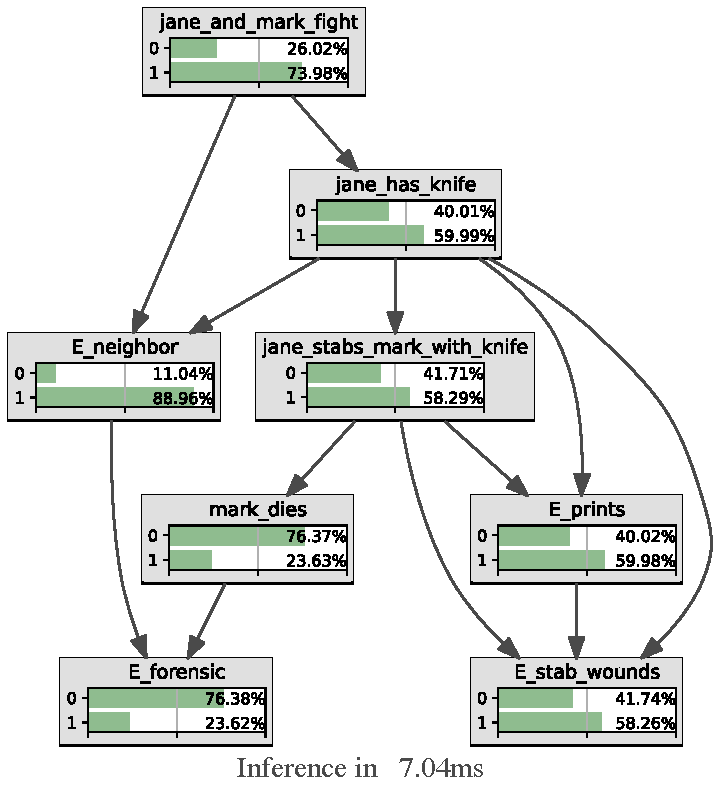
\includegraphics[width=\linewidth]{../experiments/WalkThrough/bnImage/BNIMAGEWalkThrough.pdf}
\caption{Walkthrough network.}
\label{genepool}
\end{figure}
\end{example}

After the network is generated, we need to manually change a thing about it. The algorithm does not know how to handle impossible states, which are cases where combinations of valuations for parent nodes are impossible. For example, in Figure~\ref{genepool}, the value of `E\_forensic'. `E\_forensic' has two parents: `mark\_dies', as well as `E\_neighbour'. In the simulation, it can never be the case that Mark dies, but the neighbour does not hear and report on fighting, or the combination of events $`mark\_dies' \rightarrow 1 \land `E\_neighbour' \rightarrow 1$ .  However, the event for the thief stealing the object, can have both `motive' and `knowing about object' as parent nodes. The algorithm does not know how to deal with these situations and the resulting network will crash. This is why the probability for `stealing' given the impossible combination of the parent state values, will be manually set to 0. 


\section{Evaluating the Bayesian Network}

Now we know that we can build Bayesian Networks automatically using the K2 algorithm based on data we generated in our simulation, we need to evaluate different aspects of the Bayesian Network.


\subsection{Numbers}
\begin{enumerate}
\item \textbf{Do the conditional frequencies in the BN correspond to the conditional frequencies in the simulation?}
\item \textbf{Could you find the numbers?}
\item \textbf{How robust are the BNs to reduced precision in the CPTs?}
\end{enumerate}

\subsection{Structural}

\begin{enumerate}
\item \textbf{Does the BN represent all relevant events of the scenario?}
\item \textbf{Does the BN have temporal ordering of the hypothesis nodes?}
\item \textbf{Does the BN follow the evidence-idioms (evidence not parents of hypothesis nodes)?}
\item \textbf{Can the BN represent multiple alternative scenarios?}

\end{enumerate}

\subsection{Predictive}
\begin{enumerate}
\item \textbf{How does the BN respond to evidence?}
\item \textbf{When does the BN predict the wrong outcome?}
\end{enumerate}
